\chapter{Heritage}
\label{chap:heritage}
\graphicspath{{Mission_Heritage/Images/}}

In the past, there have been multiple spacecraft missions to the small bodies in our Solar System which have collectively increased our understanding about them. While a large majority of these have been asteroid fly-by scenarios, a few have also been rendezvous missions \parencite{esa_mission2asteroids_web}. This chapter will provide an overview on a few of these missions, followed by a brief literature review which shall be of interest to the thesis at hand. This will help us in justifying the research objectives mentioned in \Cref{chap:research_questions}. \Cref{sec:past_missions} will discuss the asteroid rendezvous missions which have already taken place, \Cref{sec:future_missions} will discuss future rendezvous missions, and finally \Cref{sec:literature_review} will discuss the state-of-the-art.

\section{Past Missions}
\label{sec:past_missions}
In all history of space exploration there have been only three spacecraft missions that have rendezvoused with asteroids. In chronological order these are: \gls{NASA}'s \gls{NEAR}-Shoemaker mission to asteroid Eros, \gls{JAXA}'s Hayabusa mission to asteroid Itokawa, and \gls{NASA}'s Dawn mission to asteroids Vesta and Ceres \parencite{scheeresBook}. Out of these, only \gls{NEAR} and Hayabusa had direct contact with the small bodies and acquired high-resolution imagery of surface regolith.

\subsection{NEAR-Shoemaker}
\label{subsec:near_heritage}
The \gls{NEAR}-Shoemaker (henceforth \gls{NEAR}) mission was launched in 1996 and rendezvoused with Eros in 2000. Its operational phase around the asteroid continued for about a year during which it obtained several high-resolution images of the surface and collected comprehensive measurements to estimate its internal mass distribution, shape model, gravity and spin state amongst other observations \parencite{scheeresBook}. The bulk density of Eros was estimated to be $2.67 \pm 0.03$ \si{\gram\per\centi\metre\cubed} and its mass to be $(6.6904 \pm 0.003) \times 10^{15}$ \si{\kilo\gram}. The rotation state was estimated to be $1639.38922 \pm 0.00015$ deg/day which gives a rotational period of about $5.27$ hours \parencite{erosShapeDetermination}. On 25 October 2000, \gls{NEAR} executed a \gls{LAF} over Eros in which it acquired several high-resolution images that helped in understanding the surface morphology. The images confirmed the existence of a substantial amount of regolith on the surface with a typical thickness of tens of metres over the bedrock, except on steep slopes. The regolith was found to be highly complex, in that it varied from fine material to metre-sized ejecta blocks \parencite{Veverka2001}. \cite{Robinson2001} estimates the size of the finer regolith to be around 1.0 \si{\centi\metre} or smaller from images that had a resolution of 1.2 \si{\centi\metre} per pixel. \Cref{fig:eros_regolith} depicts the regolith morphology in one of the high-resolution imaging sequences from the \gls{LAF} \parencite{veverka2001landing}.
%%%
\begin{figure}[htb]
\centering
\captionsetup{justification=centering}
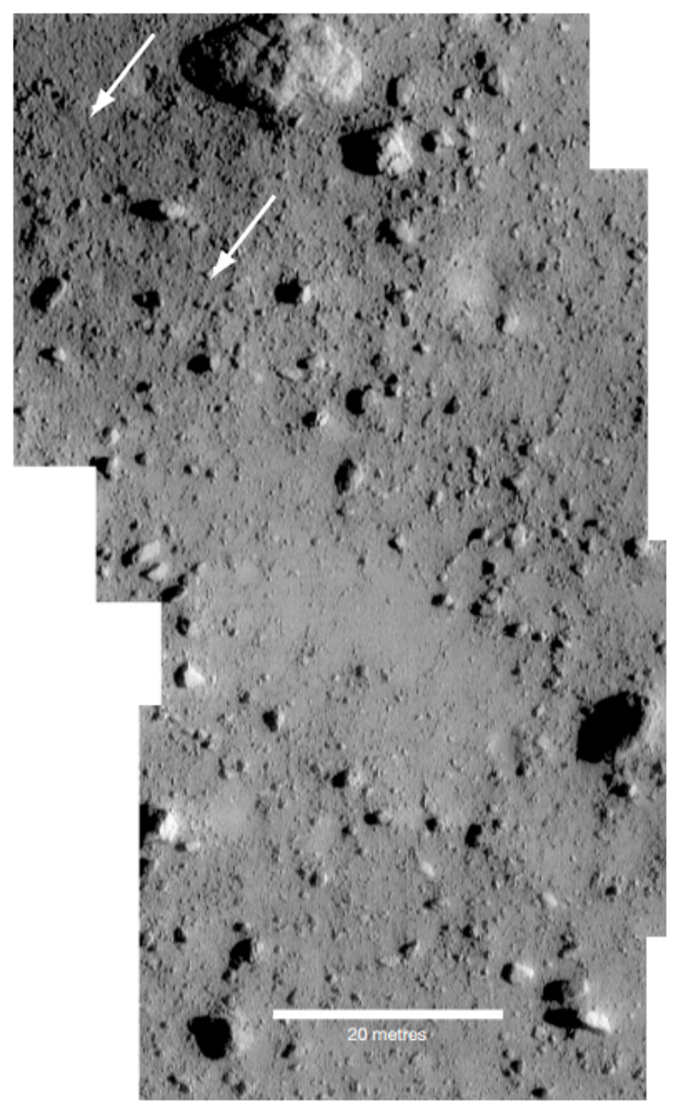
\includegraphics[width=\linewidth, height=0.5\textheight, keepaspectratio=true]{eros_regolith.pdf}
\caption{Mosaic of high-resolution images depicting the nature of regolith on the surface of Eros. The arrows in the image point to the region for which zoomed-in images are available but are not shown in this report. They can be found in \cite{veverka2001landing}.}
\label{fig:eros_regolith}
\end{figure}
\FloatBarrier
%%%

\subsection{Hayabusa}
\label{subsec:hayabusa_heritage}
The Hayabusa spacecraft was launched by \gls{JAXA} in 2003 and it arrived at asteroid Itokawa in 2005. After arrival, it performed close-proximity operations around the asteroid for approximately three months during which several measurements were taken to estimate the shape, mass, topography and elemental composition of the asteroid. During this period, the spacecraft also collected samples from the surface of the asteroid that were eventually returned back to Earth in 2010. The measurements at Itokawa estimated its mass to be $3.51 \times 10^{10}$ \si{\kilo\gram} and its bulk density to be $1.9 \pm 0.13$ \si{\gram\per\centi\metre\cubed} \parencite{fujiwara2006ItokawaHayabusa}.
%
\newline\newline
%
Two distinct types of terrain can be recognized on Itokawa; one which is rough and rich in boulders and the other which is smooth and mostly flat. This distinction can easily be seen in \Cref{fig:itokawa_regolith}. The smooth regolith regions, that account for approximately 20\% of Itokawa's surface, are composed of fragmented debris with grain sizes ranging from sub-centimetre to centimetre scales. One of the smooth regolith regions, called Muses Sea and from where the sample was also acquired, even consisted of a few metre-sized boulders that were hypothesized to have landed in the region as secondary ejecta \parencite{miyamotoItokawaRegolith}. The rougher terrain on Itokawa, which has a very sharp boundary with the smoother regolith filled regions (as evident in \Cref{fig:itokawa_regolith}), consists of boulders that range upto tens of metres in size \parencite{fujiwara2006ItokawaHayabusa}.
%%%
\begin{figure}[htb]
\centering
\captionsetup{justification=centering}
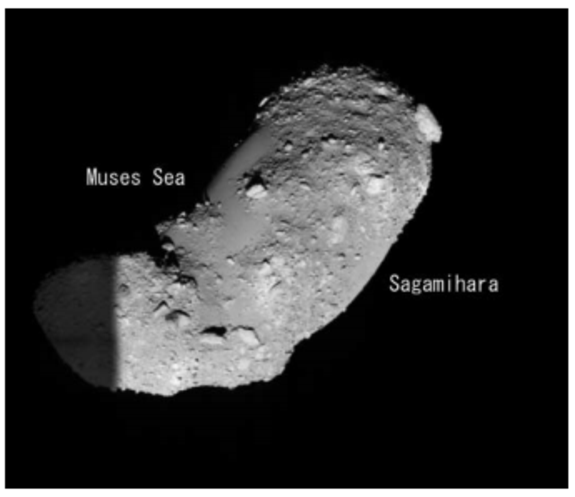
\includegraphics[width=\linewidth, height=0.4\textheight, keepaspectratio=true]{itokawa_regolith.pdf}
\caption{Image of Itokawa taken from a 7 \si{\kilo\metre} altitude depicting the nature of regolith on its surface. Muses Sea and Sagamihara are two distinct smooth regolith regions on the asteroid \parencite{fujiwara2006ItokawaHayabusa}.}
\label{fig:itokawa_regolith}
\end{figure}
\FloatBarrier
%%%
Hayabusa employed an impact sampling mechanism that would work across various types of terrains, from hard bedrock to fine regolith. The spacecraft consisted of a long cylindrical sampling horn with a conical tip. When the tip of the horn touched the surface of the asteroid, the deformation in the horn's fabric was detected by a laser range finder and within 0.3 \si{\second} of this event, a 5.0 \si{\gram} projectile was fired towards the surface with a velocity of 300 \si{\metre\per\second} and the resultant ejecta was collected by the sampler \parencite{yano2004sampling}. \cite{yanoHayabusaTouchdown} presents data from the sampling experiments that were performed on ground in 1.0 \si{\gram} and micro-gravity environments. The experiments revealed that, for the projectile hitting at normal impact angles in micro-gravity, the impact ejecta mass of particles greater than 1.0 \si{\centi\metre} ranged from 2 - 11 \si{\gram} whereas for particles less than 1.0 \si{\milli\metre} the ejecta mass ranged from 100 - 10000 \si{\gram}. The impact target consisted of various analog materials from glass beads to lunar regolith simulant and an experiment like this is a nice indicator of how artificial impact events can displace significant amount of fragmented debris on an asteroid.

\section{Future Missions}
\label{sec:future_missions}
We will now discuss two missions, Hayabusa-2 by \gls{JAXA} and \gls{OSIRIS-REx} by \gls{NASA}. Both are currently en route to their respective target asteroids and after orbit insertion, they shall perform operations to collect surface samples.

\subsection{Hayabusa-2}
\label{subsec:hayabusa2_heritage}
Hayabusa-2 is the second asteroid sample return mission by \gls{JAXA}, which to a significant extent shares the successful technical legacy of Hayabusa. The target asteroid of the former is 1999 JU3 which is suspected to contain organic matter and hydrated minerals \parencite{TsudaHayabusa2SystemDesign}. A shape model of the asteroid, also designated as Ryugu, is shown in \Cref{fig:ryugu_shape} \parencite{ryuguShapeModel}. A successful sample return from this asteroid may thus help us in understanding the origin of life and/or water on Earth. The spacecraft will enter into an orbit around its target by mid-2018, after which it will perform close-proximity operations for 1.5 years. The mission will entail three touchdowns for sample acquisition and a cratering event to observe the subsurface of the asteroid. The sampling mechanism is based on that of Hayabusa and each sampling attempt has the potential to acquire samples in the order of 100 \si{\milli\gram}. The samples are sealed-off and transported back to Earth in a re-entry capsule. The cratering operation is performed by a \gls{SCI}. The \gls{SCI} is deployed by the spacecraft at an altitude of 500 \si{\metre} and after a preset time, a detonation accelerates it to about 2 \si{\kilo\metre\per\second} prior to impact. It is estimated that this will result in a crater of about 2 \si{\metre} wide. Prior to the detonation of \gls{SCI}, the spacecraft will move to a safe location on the opposite side of the asteroid from the impact point to avoid damage from impact ejecta and/or debris from the detonation. Apart from these, the spacecraft will perform other in-situ operations to characterize the asteroid and will also deploy a lander and three miniature rovers for technology demonstration \parencite{TsudaHayabusa2SystemDesign}.
%%%
\begin{figure}[htb]
\centering
\captionsetup{justification=centering}
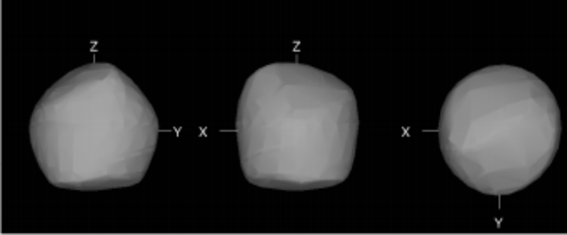
\includegraphics[width=\linewidth, height=0.3\textheight, keepaspectratio=true]{ryugu_shape.pdf}
\caption{Ryugu shape model as estimated from the observations made by Herschel Space Observatory, supported by several ground-based measurements and data from other space-based assets \parencite{ryuguShapeModel}.}
\label{fig:ryugu_shape}
\end{figure}
\FloatBarrier
%%%

\subsection{OSIRIS-REx}
\label{subsec:osiris_heritage}
\gls{OSIRIS-REx} is part of \gls{NASA}'s New Frontiers program and will travel to \gls{NEA} 1999 $RQ_{36}$, also known as Bennu. A shape model of the asteroid is shown in \Cref{fig:bennu_shape} \parencite{bennuShapeModel}. The mission, amongst other scientific objectives, will return a regolith sample back to Earth that may provide insight into the initial states of planetary formation as well as answer questions on the origins of life. Since Bennu is a \gls{NEA}, the sample collection and subsequent analysis will provide us information on asteroids that could potentially impact Earth. The spacecraft was launched in 2016 and is expected to reach its target by the end of 2018 \parencite{berry2013osiris}. The asteroid has a semi-major axis of 1.126 AU which makes it an easily accessible asteroid as far as distance is concerned. But more than that, Bennu falls under the category of asteroids that are rich in volatiles and could potentially be related to objects that brought the seeds of life to Earth. Initial observations of Bennu through ground-based telescopes, the Spitzer Telescope, the Arecibo Observatory and other assets revealed an abundance of regolith on the surface with grain sizes ranging from 4 - 8 \si{\milli\metre}. \gls{OSIRIS-REx} will acquire the regolith sample using a \gls{TAG} mechanism which uses pressurized nitrogen gas to force the loosely-held regolith into a collection chamber. The sampling will occur in 2020 and it will be retrieved on Earth in 2023 \parencite{osirisMissionOverview}.
%%%
\begin{figure}[htb]
\centering
\captionsetup{justification=centering}
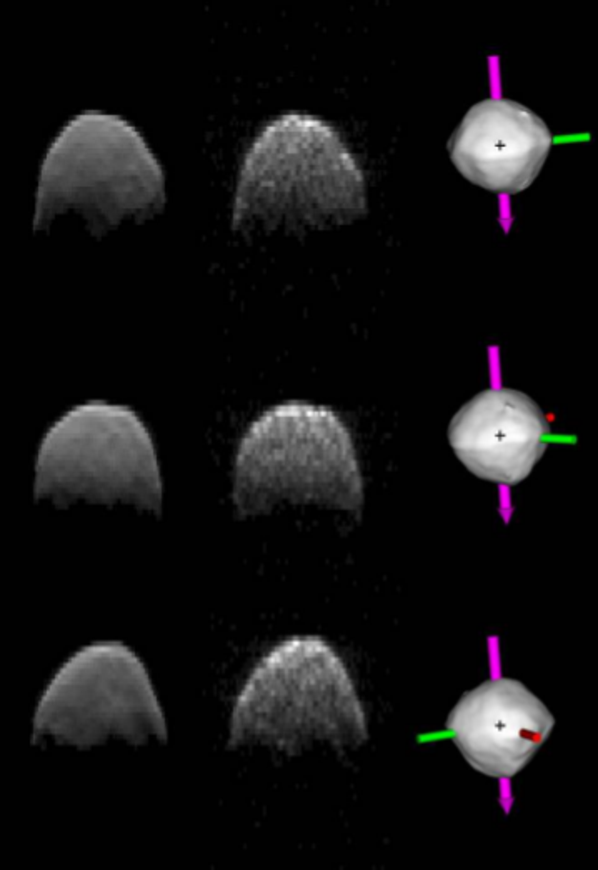
\includegraphics[width=\linewidth, height=0.4\textheight, keepaspectratio=true]{bennu_shape.pdf}
\caption{Bennu's shape as observed from the radar data collected by the Goldstone and Arecibo observatories (shown in middle column of the image). The left column displays the model that provides the best fit to the radar data and the right column shows the final estimated 3D model of Bennu as it would appear in the sky \parencite{bennuShapeModel}.}
\label{fig:bennu_shape}
\end{figure}
\FloatBarrier
%%%

\section{State of the art / Literature Review}
\label{sec:literature_review}
In this section we shall discuss a few research papers relevant to this thesis; the techniques they applied to understand the orbital behavior of impact ejecta and the shortcomings of these studies.
%
\newline\newline
%
A good starting point to understand the topic at hand is provided by \cite{scheeres2002fate}. It reviews the gravity and perturbing force models along with the dynamical equations of motion for a particle in orbit around an asteroid and the model for generating initial conditions to launch ejecta from the surface of an asteroid. It also mentions existing analytical methods to compute guaranteed escape and re-impact speeds for impact ejecta i.e. speeds at which particles would immediately escape or re-impact after being launched. \cite{scheeres2002fate} also discusses the various numerical and analytical methods that have been used in literature for analyzing the motion of particles that stay in pseudo-stable orbits for extended periods of time before meeting their final fate. It also presents various mechanisms that have been hypothesized for the capture-case scenario i.e. particles that stay in orbit around asteroids for a relatively long time, from hundreds of days to several years. The analysis of these capture orbits, in particular, has been done by considering the Solar perturbations and irregular gravity effects of the asteroid but always in isolation.
%
\newline\newline
%
\cite{richter1995stability} provides an analytical method to solve for the motion of particles around a non-rotating, spherical cometary nucleus which is in an eccentric, heliocentric orbit. In their paper, they ignore Solar tidal effects and assume that the particle motion around a homogeneous spherical body would experience weak perturbations from \gls{SRP}. They give averaged equations for the variation of eccentricity and angular momentum vectors as a function of the true anomaly of the comet around the Sun. The paper also discusses the limitations and validity of using their analytical approximation as well as the conditions for collision-free orbits for small and large dust particles around the comet. Although the study conducted by \cite{richter1995stability} is for comets, it can be extended to asteroids as well and has been used by \cite{morrow2001solar} for analyzing solar sail powered trajectories around them. \cite{lee1996dust} discusses the electrostatic levitation of dust particles from the surface of an asteroid. It uses two electrostatic field production methods used in the study of dust levitation on a moon, and applies them to the case of an asteroid. The study does not involve the orbital motion of dust particles but it does provide conditions which could cause the dust particle to escape in the event of electrostatic levitation.
%
\newline\newline
%
\cite{scheeres1996orbits} provides an extremely detailed and systematic study of particle dynamics close to the surface of asteroid Castalia. They include the effect of the irregular shape of the asteroid on orbital dynamics by using a spherical harmonics model of degree and order upto four in simulating the gravity potential. They also derive analytical results for the computation of guaranteed return and escape speeds as a function of the location of a particle on the surface of the asteroid. The paper employs dynamical systems theory and investigates the use of stable manifolds associated with orbits around equilibrium points and intersecting the surface of the asteroid, to obtain the initial launch conditions for the particle that will lead to a temporary stable orbit around the asteroid. \cite{scheeres2000ejecta} applies the radiation pressure approximation method developed by \cite{richter1995stability} to study the temporary capture of particles in an orbit around a comet, but improves it to account for the comet's rotation as well. The results obtained from the analytical approximation are compared with the results from the numerical simulation wherein the latter accounts for other perturbations as well such as Solar tidal effects and gravity field variations. The comparison showed that the radiation pressure approximation method by \cite{richter1995stability} is qualitatively correct and can be used for statistical studies at the very least. They were also able to establish qualitative ranges on ejecta velocity and angles that result in capture orbits, an example of which is shown in \Cref{fig:comet_temporary_capture_example}.
%%%
\begin{figure}[htb]
\centering
\captionsetup{justification=centering}
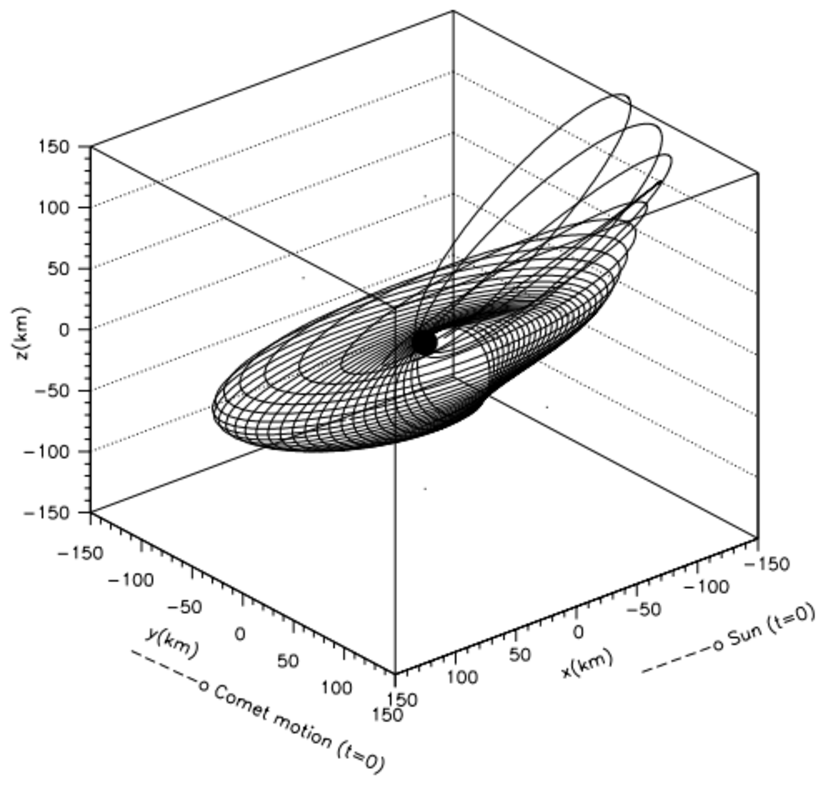
\includegraphics[width=\linewidth, height=0.4\textheight, keepaspectratio=true]{capture_orbit_tempel1_scheeres.pdf}
\caption{Example of a single particle capture trajectory around comet Tempel-1 \parencite{scheeres2000ejecta}.}
\label{fig:comet_temporary_capture_example}
\end{figure}
\FloatBarrier
%%%

\cite{korycansky2004_impactEjecta} conducts a study to understand the distribution of impact ejecta and its connection with existing regolith on the surface of asteroid 433 Eros. The study involves the use of a Monte Carlo simulation technique to observe the orbital evolution of a large number of test particles from randomly selected locations on the asteroid. They use a coarse polyhedron model of asteroid Eros to model its gravitational field, thus accounting for gravity perturbations. However, the research does not account for perturbations from \gls{SRP}. \cite{yarnoz2014passive} studies the orbital motion of lofted regolith in the context of using \gls{SRP} to passively sort asteroid material. They use semi-analytic methods to derive conditions that would cause regolith to either escape or re-impact the asteroid’s surface. They make use of the radiation pressure approximation methodology developed by \cite{richter1995stability} in their semi-analytical approach. However, the effect of an irregular shape of an asteroid, i.e. gravity perturbations, is not accounted for in their calculations.
%
\newline\newline
%
In general, we witnessed minor drawbacks in these studies such as not always accounting for gravity and Solar perturbations together, or the derivation of an analytical solution which is not globally valid. Some studies involved both analytical and numerical methods for simulating orbital dynamics but even then the numerical approach was more for comparing the validity of the analytical solution and not as much for obtaining the full range of initial conditions that will lead to re-impact, escape or temporary capture of regolith around an asteroid. The effect of launch direction of regolith was also not considered in most of the studies, especially the ones that applied analytical methods. We attempt to address these shortfalls to better understand the reasons for the complex orbital behavior of particles launched from the surface of an asteroid, by following a numerical simulations approach instead of an analytical approximation or a dynamical theory one (see \cite{scheeres2002fate} for a brief discussion between the three methods for analyzing orbital behavior of asteroid ejecta). We account for gravity and Solar perturbations while simulating trajectories for particles of different sizes and density. These perturbations have been considered in isolation as well as together to witness the effect of each individual perturbation on a particle trajectory.

